\documentclass[10pt]{article}
\usepackage{amsmath, amsthm, amsbsy, rotating,float}
\usepackage{graphicx,algorithm,algorithmic,subfig}
\usepackage{setspace,enumerate}
\doublespacing




\author{Esteban D\'{i}az}
\title{Homework 4}{}

\begin{document}
\maketitle

I did the stem and leaf plot counting the hits every
two hundred $cc$ of rainfall. In this way the plot does
not seem sparse. One can see that most of the rainfall
is located around $(800-1000)cc$. The distribution 
seem to have a non normal shape with a long tail decay.
One can see 1 very obvious outlier.

\begin{verbatim}
  4|23799                22| 
  6|4557                 24|7  
  8|2224557889           26|235
 10|569                  28|
 12|1667899              30|
 14|3788                 32|
 16|5569                 34| 
 18|0223                 36| 
 20|0                    38|1
\end{verbatim}



\begin{figure}[H]
    \centering
    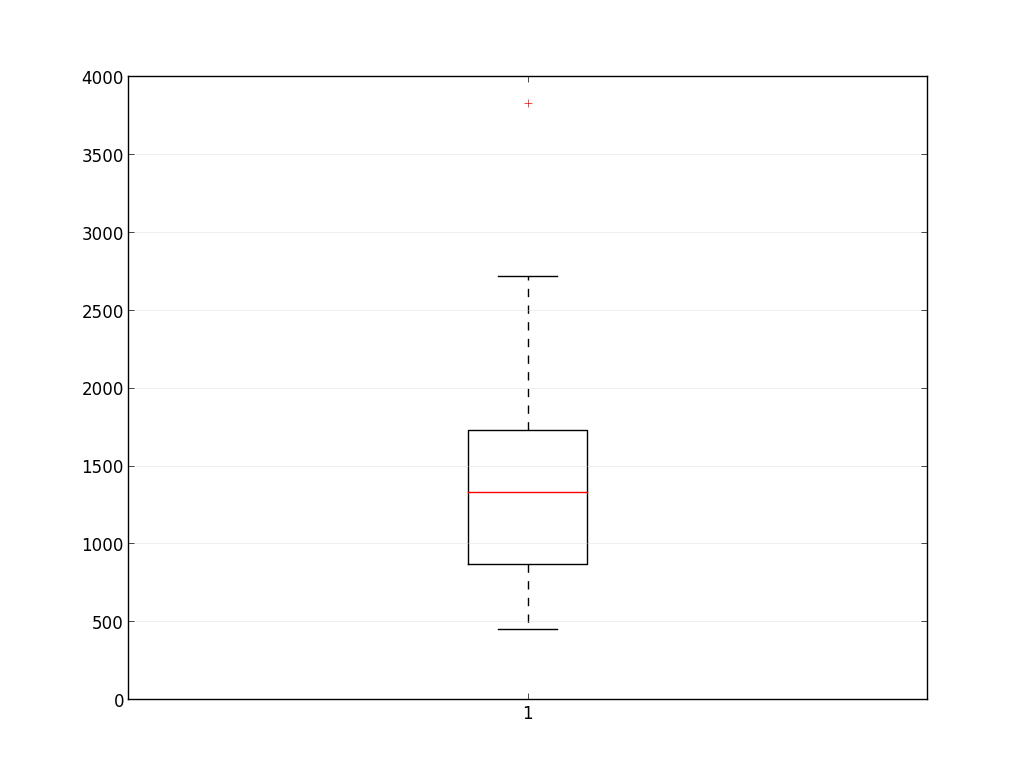
\includegraphics[width=0.85\textwidth]{boxplot.png}
    \caption{Box plot of the rainfall data. There is one outlier outside the criterion 1.5xIQR rule (3830)}
    \label{fig:fig1}
\end{figure}

\begin{figure}[H]
    \centering
    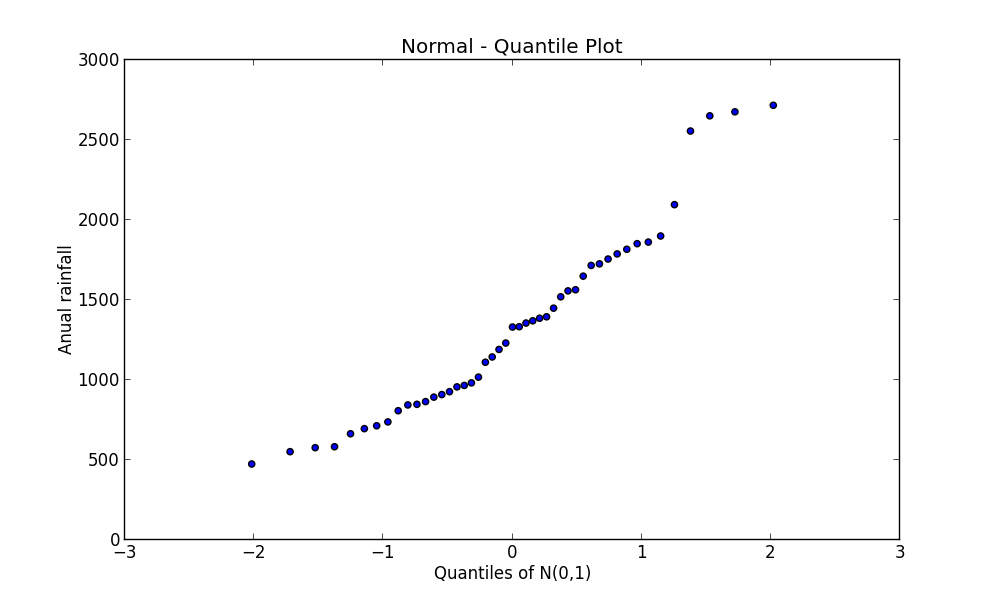
\includegraphics[width=0.85\textwidth]{qqplot.png}
    \caption{QQ plot of the rainfall data. One can see that the distribution  is skewed towards the high values of rainfall (i.e. if one removes the 5 highest values, then the distribution could be approximated to a normal). }
    \label{fig:fig2}
\end{figure}

\end{document}
